\subsubsection{Preconsiderations}
There exists only a few public 4k video databases. They differ in content (scenario, field size, camera movement, illumination condition) as well as in technical aspects (resolution, frame rate, bit rate and color bit depth). 
To obtain reference video files for the subjective test, parts of the 4k content from the databases are used (also called source video files).
For our test we want to have a large variety between the reference video files to evoke different encoding properties. 
All the reference videos should have a duration of 10 seconds with no cuts inside.
To avoid the influence of judder, the smallest permitted frame rate of the source videos is 50 frames per second (fps). Furthermore the smallest resolution considered to be 3840x2160. If the source videos are not 4k (4096x2160 pixels) they will be upscaled before distortion. Moreover the frame rate of the reference video files is being adapted to consistent 50fps.
\newline

\subsubsection{Dataset Preparation}
For obtaining a good variety of video sequences three data bases are used: The Harmonic \cite{web:harmonic} which contains 18 different video files, Cable Labs \cite{web:cablelabs} with 9 relevant 4k contents and the Blender Foundation \cite{web:bbb} for receiving the cartoon Big Buck Bunny. They  are partial under the creative commence license and all of them are available in the ProRes format, except of Big Buck Bunny where the 4k video content can be downloaded only as a compressed video file, however there also exist high quality PNGs for all the frames of the cartoon. In order to generate a high quality reference video with the frames of Big Buck Bunny, an automatisation script is used to find a sequence with a duration of 10 seconds, to download the respective images and to encode them as a video file.
Generally, the challenge is to extract 10 seconds sequences from the original video files with no cut inside because there exists only a few.

One problem of the video sequences from the database is that even they have a high bit rate and are stored as ProRes, no conclusion referring to the contained visual quality can be done. 
For this reason a preselection with a very powerful system, able to play 4k content in ProRes with high bit rates and connected to a 4k screen, was applied.
The remaining reference videos are 6 source clips, each with a duration of 10 seconds. All the files have got a resolution of 3840x2160 pixels and are stored in the ProRes format. Because this format is a 10 bit codec only, the original color depth of each video file can not be determined.
Further specific informations about the reference videos are shown in Table \ref{tab:Specifications}.

\begin{table}[!t]
	\renewcommand{\arraystretch}{1.3}
	\centering
	\caption{Meta data of the video files. The timestamps are the start positions of the extraction of 10 second sequences from the source files, where m stands for minutes, s for seconds and ms for milliseconds respectively. Further shortcuts: H = Harmonic, B = Blender Foundation, C = Cable Labs}
	\label{tab:Specifications}
	\begin{tabular}{lcccc}
		%\cline{2-6}
		\toprule
		Sequence Name       & Frame Rate & Bit rate & Timestamps & Source\\
							& fps  	   & Mbits/s    & mm:ss.ms   & \\
		\midrule
		Air Show            & 59.94    & 1703 & 00:48.500  &   H  \\
		Big Buck Bunny      & 60       & 2304 & 05:47.000  &   B  \\
		Fjord               & 50       & 1469 & 00:21.000  &   H  \\
		Moment of Intensity & 59.94    & 1822 & 02:16.000  &   C \\
		Snow Monkeys        & 59.94    & 1750 & 00:17.000  &   H  \\
		Streets of India    & 50       & 2094 & 00:00.000  &   H  \\
		\bottomrule
	\end{tabular}
\end{table}

They contain a wide range of high-level features (animation, camera motion, people, water) and low-level characteristics (brightness, contrast, texture, motion, color variance, sharpness) as can be seen in Figure \ref{fig:OverviewReferenceSequences}.

\begin{figure}[h]
	\begin{center}
		%

		\subfigure[Air Show]{%
			\label{fig:airshow}
			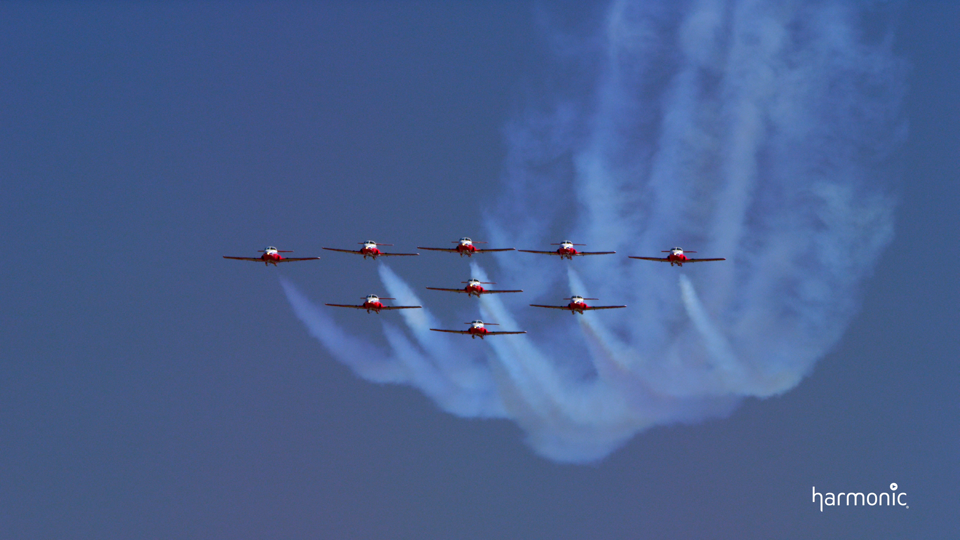
\includegraphics[width=0.2\textwidth]{images/AirShow}
		}%
		\subfigure[Big Buck Bunny]{%
			\label{fig:bbb}
			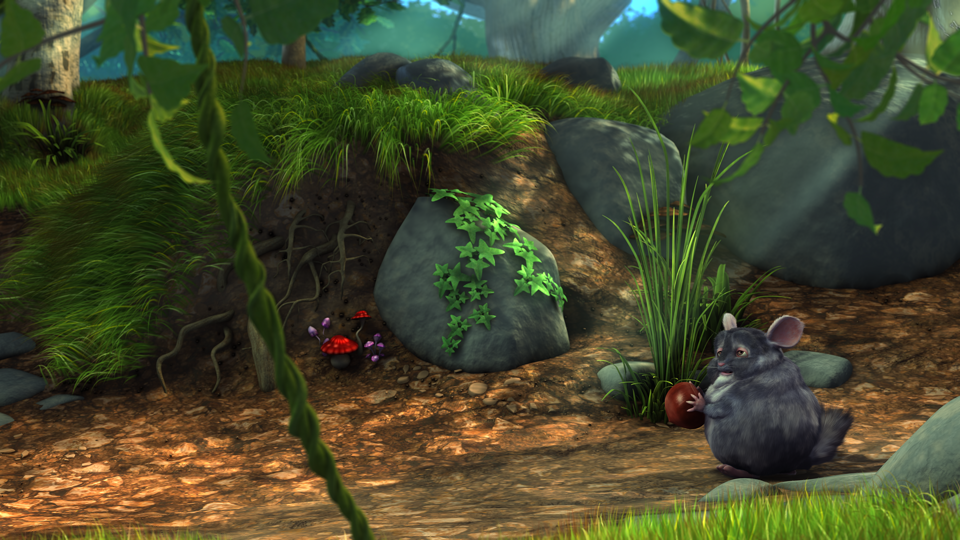
\includegraphics[width=0.2\textwidth]{images/Bbb}
		}\\ %  ------- End of the first row ----------------------%
		\subfigure[Fjord]{%
			\label{fig:Fjord}
			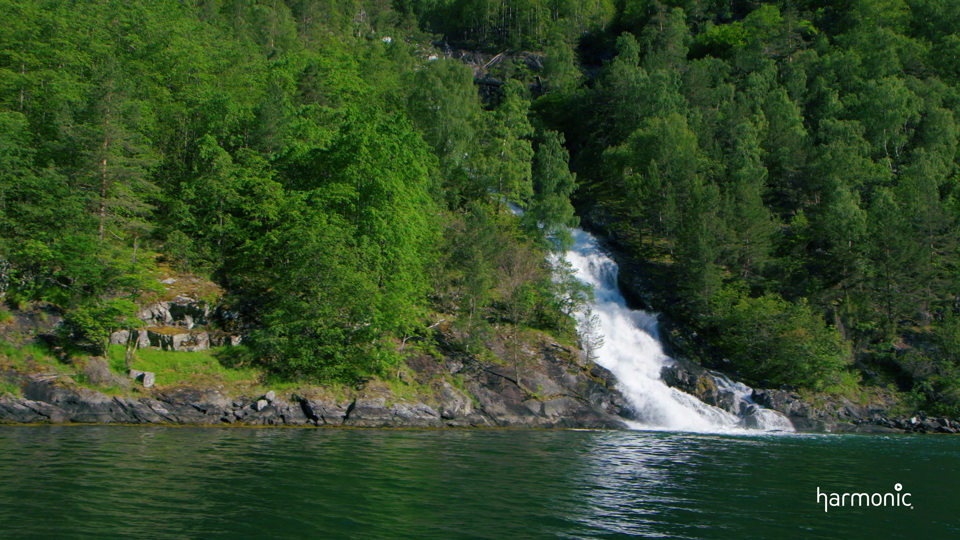
\includegraphics[width=0.2\textwidth]{images/Fjord}
		}%
		\subfigure[Moment of Intensity]{%
			\label{fig:MomentOfIntensity}
			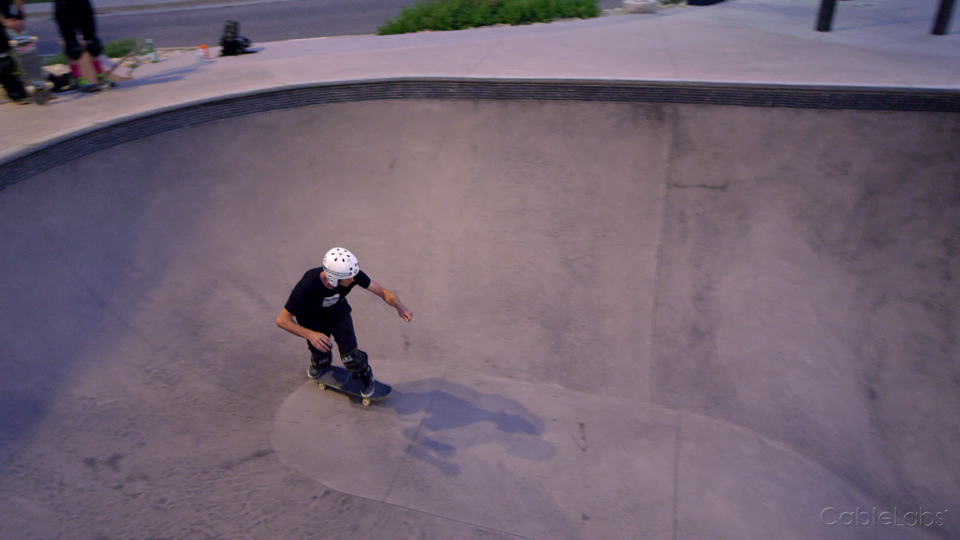
\includegraphics[width=0.2\textwidth]{images/MomentOfIntensity}
		}\\ %  ------- End of the second row ----------------------%		
		\subfigure[Snow Monkeys]{%
			\label{fig:SnowMonkeys}
			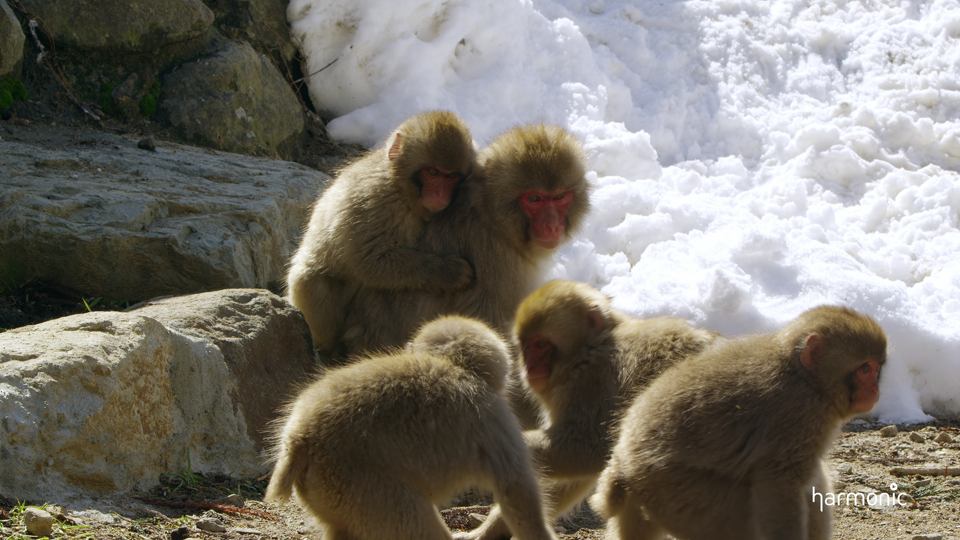
\includegraphics[width=0.2\textwidth]{images/SnowMonkeys}
		}%
		\subfigure[Streets of India]{%
			\label{fig:StreetsOfIndia}
			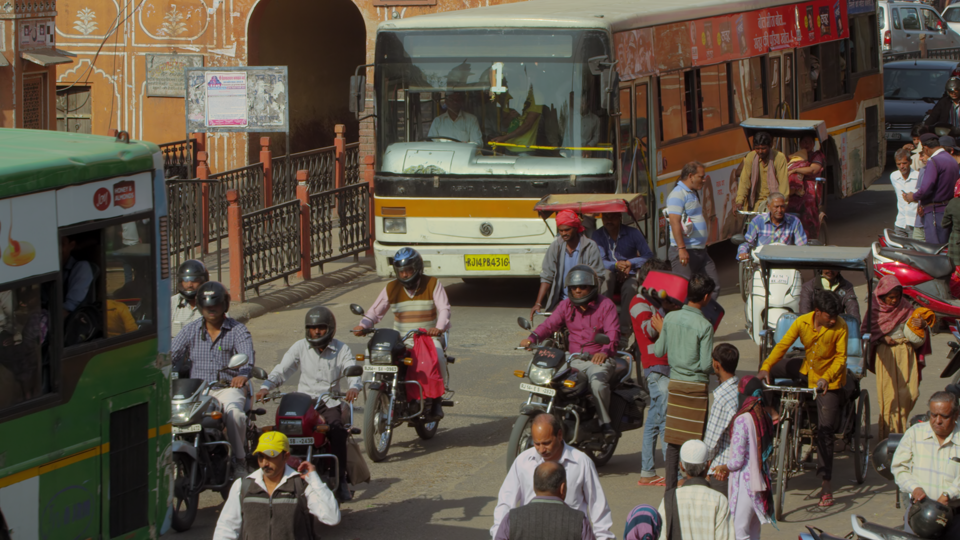
\includegraphics[width=0.2\textwidth]{images/StreetsOfIndia}
		}%
		%
	\end{center}
	\caption{%
		Selection of frames contained in the reference videos to show the variety of the content.
	}%
	\label{fig:OverviewReferenceSequences}
\end{figure}

